%%%%%%%%%%%%%%%%%%%%%%%%%%%%%%%%%%%%%%%%%%%%%%%%%%%%%%%%%%%%%%%%%%%%%%%%%%%%%%
% OPTCON-RL 2025/2026 - Course Project #2
% Optimal Control of a Flexible Robotic Link
%
% File:         OPTCON_report_template_.tex
% Description:  LaTeX template for the OPTCON-RL course project report.
%
% Authors:      Francesco Cenni, Giulio Mazzaroppi, Giacomo Pezzolati
% Affiliation:  Alma Mater Studiorum Università di Bologna
% Date:         December 2025
%%%%%%%%%%%%%%%%%%%%%%%%%%%%%%%%%%%%%%%%%%%%%%%%%%%%%%%%%%%%%%%%%%%%%%%%%%%%%%

%----------------------------------------------------------------------------------------
%	DOCUMENT CLASS
%----------------------------------------------------------------------------------------
\documentclass[a4paper,11pt,oneside]{article}

%----------------------------------------------------------------------------------------
%	PACKAGES
%----------------------------------------------------------------------------------------
\usepackage[utf8]{inputenc}                     % UTF-8 encoding
\usepackage[T1]{fontenc}                        % Font encoding
\usepackage{amsmath, amssymb, amsthm}           % For mathematical symbols and environments
\usepackage{graphicx}                           % Essential for inserting images/figures
\usepackage{geometry}                           % For setting page dimensions and margins
\usepackage{float}                              % Improved interface for floating objects
\usepackage{subcaption}                         % For subfigures
\usepackage{listings}                           % For including code snippets
\usepackage{xcolor}                             % For defining colors
\usepackage{hyperref}                           % For hyperlinks in the document
\usepackage{booktabs}                           % For professional looking tables
\usepackage{siunitx}                            % For typesetting units and quantities
\usepackage[english]{babel}                     % Sets language rules for hyphenation and titles
\usepackage{color}                              % Allows the use of colored text/boxes
\usepackage{cite}                               % Manages bibliographic citations in the text
\usepackage{graphicx}                           % Essential for inserting images/figures
\usepackage{float}                              % Improved interface for floating objects 
\usepackage{bm}                                 % For bold mathematical symbols (useful for vectors)
\usepackage{multicol}                           % For multiple columns layout
\usepackage{abstract}                           % For customizing the abstract section
\usepackage{cancel}                             % For striking out terms in equations
\usepackage{booktabs}                           % For professional looking tables
\usepackage{siunitx}                            % For typesetting units and quantities

%----------------------------------------------------------------------------------------
%     DOCUMENT SETTINGS
%----------------------------------------------------------------------------------------
% Margins
\geometry{
      left=25mm,
      right=25mm,
      top=25mm,
      bottom=25mm,
}

% Code Listing Style
\definecolor{codegreen}{rgb}{0,0.6,0}
\definecolor{codegray}{rgb}{0.5,0.5,0.5}
\definecolor{codepurple}{rgb}{0.58,0,0.82}
\definecolor{backcolour}{rgb}{0.95,0.95,0.92}

% Listings settings
\lstdefinestyle{mystyle}{
      backgroundcolor=\color{backcolour},   
      commentstyle=\color{codegreen},
      keywordstyle=\color{magenta},
      numberstyle=\tiny\color{codegray},
      stringstyle=\color{codepurple},
      basicstyle=\ttfamily\footnotesize,
      breakatwhitespace=false,         
      breaklines=true,                 
      captionpos=b,                    
      keepspaces=true,                 
      numbers=left,                    
      numbersep=5pt,                  
      showspaces=false,                
      showstringspaces=false,
      showtabs=false,                  
      tabsize=2
}

\lstset{style=mystyle}

%----------------------------------------------------------------------------------------
%	BEGIN DOCUMENT
%----------------------------------------------------------------------------------------
\begin{document}

%----------------------------------------------------------------------------------------
%	TITLE SECTION
%----------------------------------------------------------------------------------------
\begin{titlepage}
\thispagestyle{empty}                                                 
\begin{center}                                                            
      \vspace{5mm}
            {\LARGE UNIVERSIT\`A DI BOLOGNA} \\                       
      \vspace{5mm}
\end{center}
\begin{center}
\includegraphics[scale=.27]{figs/logo_unibo}
\end{center}
\begin{center}
      \vspace{5mm}
      {\LARGE School of Engineering} \\
      \vspace{3mm}
      {\Large Master Degree in Automation Engineering} \\
      \vspace{20mm}
      {\LARGE Optimal Control and Reinforcement Learning} \\
      \vspace{5mm}{\Large\textbf{Course Project 2 - Flexible Robotic Link}} \\                 
      \vspace{15mm}
\end{center}
\begin{flushleft}                                                                              
{\large Professor: \textbf{\@ Giuseppe Notarstefano}} \\        
      \vspace{13mm}
\end{flushleft}
\begin{flushright}
      {\large Students:}\\
      \vspace{3mm}
      {\large \textbf{\@ Francesco Cenni}} \\
      \vspace{3mm}
      {\large \textbf{\@ Giulio Mazzaroppi}} \\
      \vspace{3mm}
      {\large \textbf{\@ Giacomo Pezzolati}} \\
\end{flushright}        %capoverso allineato a destra
\begin{center}
\vfill
      {\large Academic year \@2025/2026} \\
\end{center}
\end{titlepage}   

%----------------------------------------------------------------------------------------
%	TABLE OF CONTENTS
%----------------------------------------------------------------------------------------
\tableofcontents
\newpage

%----------------------------------------------------------------------------------------
%	LIST OF FIGURES
%----------------------------------------------------------------------------------------
\listoffigures
\newpage

%----------------------------------------------------------------------------------------
%	MAIN CONTENT
%----------------------------------------------------------------------------------------
%----------------------------------------------------------------------------------------
%	ABSTRACT
%----------------------------------------------------------------------------------------
\begin{abstract}

This project addresses the optimal control and trajectory tracking of a flexible robotic link, modeled as an under-actuated planar double pendulum with nonlinear joint stiffness.

The goal of this work is to develop a comprehensive framework for trajectory generation and tracking control, considering the system's inherent nonlinearities and actuation constraints.

The study adopts a flexible discretization framework where the integration scheme is selected based on the specific requirements of the maneuver and its required fidelity. The analytic Jacobians are derived directly from the chosen discrete-time mapping, ensuring that the gradients remain consistent with the state-transition dynamics.

We analyze the system's equilibrium manifold to identify stable and unstable configurations. 

Trajectory generation is performed using a Newton-based approach.  Moreover, a novel Dynamic Horizon Extension strategy is proposed to enhance the convergence of trajectory optimization algorithms in the presence of complex dynamics.

Finally, we implement and compare two tracking controllers: a Linear Time-Varying Linear Quadratic Regulator (LTV-LQR) for unconstrained stabilization, and a Model Predictive Control (MPC) scheme to handle actuator saturation. 

Simulation results demonstrate the efficacy of the proposed extension strategy in generating feasible trajectories and highlight the superior performance of MPC in tracking under input constraints.

\end{abstract}
\newpage                % Abstract
%----------------------------------------------------------------------------------------
%	INTRODUCTION
%----------------------------------------------------------------------------------------


\section*{Introduction}

This report presents the design and implementation of optimal control strategies for a flexible robotic link.
The system is modeled as a planar double pendulum where only the first joint is actuated, and a nonlinear elastic behavior is present at the end of the second link.

This structure introduces significant control challenges, specifically:
\begin{itemize}
    \item \textbf{Under-actuation:} The system has two degrees of freedom (DoF) but only one control input (torque at the base);
    \item \textbf{Nonlinear Elasticity:} The stiffness between the links depends nonlinearly on the relative angle $\theta_2$, complicating the dynamics compared to standard linear springs;
    \item \textbf{Non-controllability:} The system is not fully feedback linearizable, and maintaining equilibrium requires precise balancing of gravitational and elastic forces;
    \item \textbf{Low Friction:} The provided parameters (Set 2) involve relatively low friction coefficients, making the system prone to oscillations and sensitive to disturbances.
\end{itemize}


\newpage            % Introduction
%----------------------------------------------------------------------------------------
%	SECTION 1: MODEL DISCRETIZATION
%----------------------------------------------------------------------------------------


\section{Task 0: Problem Setup and Discretization}

The continuous-time dynamics of the double pendulum are governed by the equation:
\begin{equation}
M(q)\ddot{q} + C(q, \dot{q})\dot{q} + F\dot{q} + G(q) = \begin{bmatrix} \tau \\ 0 \end{bmatrix}
\end{equation}
where $q = [\theta_1, \theta_2]^\top$. To utilize numerical optimal control techniques, these dynamics must be discretized.

\subsection{Discretization Methods}
We implemented two discretization schemes in `solver.py` to transition from continuous time $\dot{x} = f(x, u)$ to discrete time $x_{k+1} = f_d(x_k, u_k)$:
\begin{enumerate}
\item \textbf{Forward Euler (FE):} $x_{k+1} = x_k + \Delta t f(x_k, u_k)$. While simple, this method is numerically unstable for stiff systems or large time steps.
\item \textbf{Runge-Kutta 4th Order (RK4):} This method computes the state update using a weighted average of four slopes:
\begin{equation}
      x_{k+1} = x_k + \frac{\Delta t}{6} (k_1 + 2k_2 + 2k_3 + k_4)
\end{equation}
RK4 was selected as the primary method for the project due to its superior accuracy and stability preservation, which is critical for the long-horizon optimizations performed in Task 2.
\end{enumerate}

\subsection{Analytic Jacobian Computation}
For the Newton-based optimal control algorithm, accurate gradients of the dynamics are required. Relying on finite differences can introduce numerical noise, while symbolic differentiation (via SymPy) proved too slow for iterative solving.

Therefore, we implemented an \textbf{analytic Jacobian} computation in `model.py`. The Jacobians $A = \frac{\partial f}{\partial x}$ and $B = \frac{\partial f}{\partial u}$ were derived manually and implemented using optimized NumPy operations (and Numba JIT compilation for speed). This approach ensures that the linearization required for the Backward Pass in Newton's method is both precise and computationally efficient.

\newpage                % Task 0 - Problem setup
%----------------------------------------------------------------------------------------
%	SECTION 2: EQUILIBRIA ANALYSIS
%----------------------------------------------------------------------------------------


\section{Task 1: Equilibria and Terminal Cost}

\subsection{Equilibrium Manifold}
The system's equilibria are defined by states where $\dot{q} = \ddot{q} = 0$. This implies the gravity and stiffness torques must be balanced by the input $\tau$.
We analyzed the equilibrium manifold by fixing one generalized coordinate ($\theta_1$ or $\theta_2$) and solving for the other.
\begin{itemize}
\item \textbf{Elbow-Up vs. Elbow-Down:} We identified distinct configurations such as "Elbow-Up" (unstable) and "Elbow-Down" (stable).
\item \textbf{Input Requirements:} Due to the passive spring, maintaining certain angles $\theta_2$ requires a non-zero steady-state torque $\tau_{eq}$ to counteract the spring force $k(\theta_2)$.
\end{itemize}

Our analysis, visualized via the compute-equilibrium-manifold function, shows the relationship between the link configuration and the required holding torque.

\subsection{Cost Function}
For the optimal control problem, we defined the quadratic cost function:
\begin{equation}
J = \sum_{t=0}^{T-1} \left( \frac{1}{2} \Delta x_t^\top Q \Delta x_t + \frac{1}{2} \Delta u_t^\top R \Delta u_t \right) + \frac{1}{2} \Delta x_T^\top Q_T \Delta x_T
\end{equation}
where $\Delta x = x - x_{ref}$ and $\Delta u = u - u_{ref}$. We selected $Q = \text{diag}(1, 1, 1, 1)$ and $R = 10^{-3}I$ to penalize state deviation while allowing for aggressive control actions.

\subsection{Terminal Cost via DARE}
A critical aspect of the finite-horizon optimization is the terminal cost $Q_T$. Simply setting $Q_T = Q$ often fails to stabilize the system at the end of the horizon, especially for short durations.

We computed $Q_T$ by solving the \textbf{Discrete Algebraic Riccati Equation (DARE)} based on the linearization at the final target equilibrium $(x_{eq}, u_{eq})$.
\begin{equation}
P_{\infty} = A^\top P_{\infty} A - (A^\top P_{\infty} B)(R + B^\top P_{\infty} B)^{-1} (B^\top P_{\infty} A) + Q
\end{equation}
Setting $Q_T = P_{\infty}$ provides an approximation of the infinite-horizon cost-to-go. This essentially informs the solver that the trajectory continues optimally after time $T$, significantly improving convergence and stability for tasks like the "Swing Up".

\subsection{Step Size Selection (Armijo Rule)}
To ensure global convergence of the Newton method, we implemented a line search using the Armijo rule. The step size $\alpha$ is reduced ($\alpha \leftarrow \beta \alpha$) until the actual cost reduction is a sufficient fraction of the predicted reduction (based on the gradient). This prevents the solver from taking overly aggressive steps that could destabilize the trajectory.

\newpage
                % Task 1 - Equilibria analysis
%----------------------------------------------------------------------------------------
%   SECTION 3: TRAJECTORY GENERATION
%----------------------------------------------------------------------------------------

\section{Task 2: Trajectory Generation (Newton's Method)}

To generate feasible trajectories transitioning between system equilibria, we employed a Newton-type method for optimal control, specifically a Differential Dynamic Programming (DDP) approach. This method iteratively optimizes the control sequence by utilizing quadratic approximations of the cost function and linear approximations of the system dynamics to find a local minimum of the objective function.

\subsection{Reference Generation}
Given the non-convex nature of the optimization landscape, the solver requires a reasonable reference trajectory to guide convergence, even if that reference is dynamically infeasible. We analyzed two distinct generation methods:

\begin{enumerate}
    \item \textbf{Stepwise:} A naive approach involving an instantaneous switch from the initial state $x_{start}$ to the goal state $x_{goal}$. This introduces a large discontinuity in the error term, often leading to poor convergence or aggressive control spikes.
    \item \textbf{Polynomial Interpolation (Poly 5):} We generated smooth references for joint positions and velocities using 5th-order polynomials. This method ensures kinematic consistency by respecting boundary conditions (position, velocity), thereby significantly aiding the solver in finding a feasible solution.
\end{enumerate}

\begin{figure}[H]
    \centering
    % First Subfigure
    \begin{subfigure}[b]{0.8\textwidth}
        \centering
        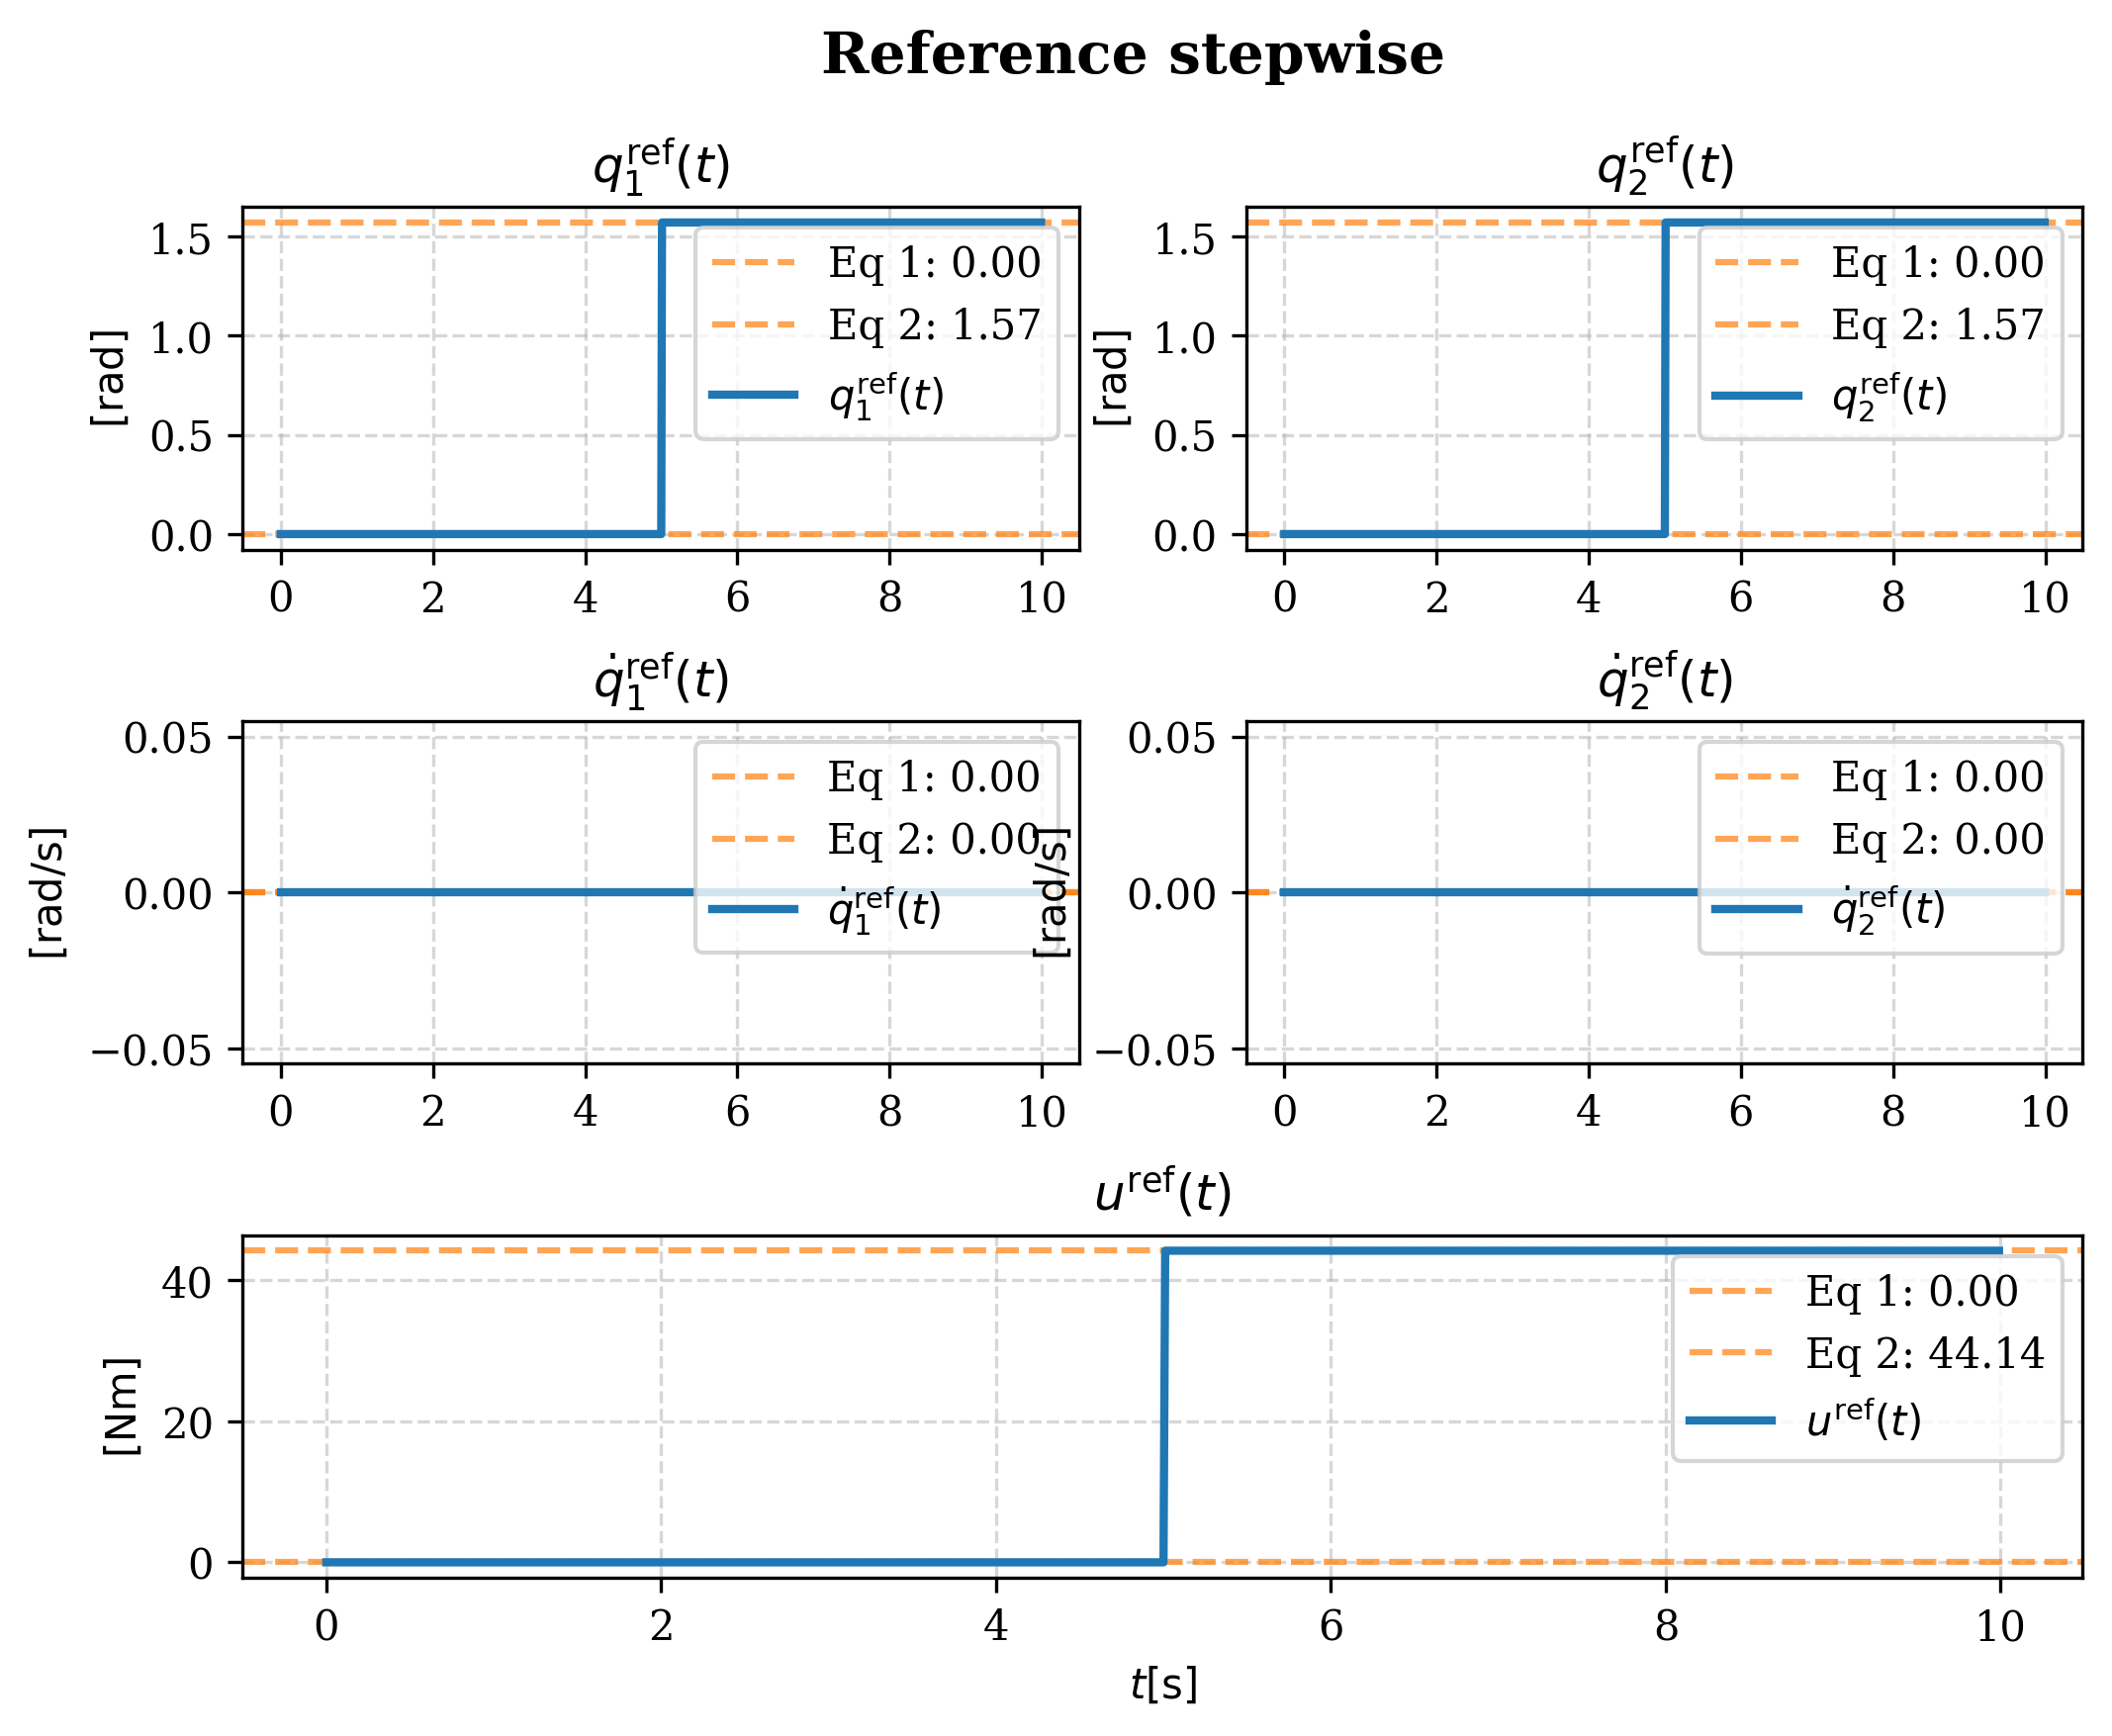
\includegraphics[width=\linewidth]{figs/misc/reference_trajectory.png}
        \caption{Stepwise Reference}
        \label{fig:ref_stepwise}
    \end{subfigure}

    \caption{Comparison of reference generation strategies.}
    \label{fig:reference_comparison}
\end{figure}


\begin{figure}[H]
    \ContinuedFloat % This command links this figure to the previous one
    \centering
    % Second Subfigure
    \begin{subfigure}[b]{0.8\textwidth}
        \centering
        \includegraphics[width=\linewidth]{figs/branch4/traj_gen_newton/elbow_up/reference_trajectory.png}
        \caption{Poly 5 Reference}
        \label{fig:ref_poly5}
    \end{subfigure}
\end{figure}


\subsubsection{Task Definitions}
We defined a set of standard maneuvers of varying complexity to evaluate the generation algorithms, ranging from simple transitions to complex swings.

\begin{figure}[H]
    \centering
    \begin{subfigure}[b]{0.5\textwidth}
        \centering
        \includegraphics[width=\linewidth]{figs/branch4/traj_gen_newton/elbow_up/double_pendulum_envelope.png}
        \caption{Elbow Up}
        \label{fig:task_elbowup}
    \end{subfigure}
    
     \begin{subfigure}[b]{0.5\textwidth}
        \centering
        \includegraphics[width=\linewidth]{figs/branch4/traj_gen_newton/swing_up/double_pendulum_envelope.png}
        \caption{Swing Up}
        \label{fig:task_swingup}
    \end{subfigure}
    
    \caption{Visualization of the defined control tasks and their target equilibria.}
\end{figure}
\begin{figure}[H]
    \centering
    \begin{subfigure}[b]{0.5\textwidth}
        \centering
        \includegraphics[width=\linewidth]{figs/branch4/traj_gen_newton/swing_down/double_pendulum_envelope.png}
        \caption{Swing Down}
        \label{fig:task_swingdown}
    \end{subfigure}
    
    \begin{subfigure}[b]{0.5\textwidth}
        \centering
        \includegraphics[width=\linewidth]{figs/branch4/traj_gen_newton/complex_maneuver/double_pendulum_envelope.png}
        \caption{Complex Maneuver}
        \label{fig:task_complex}
    \end{subfigure}
    x
    \label{fig:tasks}
\end{figure}

\subsection{Performance Analysis: Stepwise vs. Polynomial}

The choice of reference trajectory significantly impacts the solver's performance. When applying Newton's method to the \textbf{Stepwise} reference, we observed significant limitations. As seen in Figure \ref{fig:newton_stepwise}, the instantaneous jump in the reference creates a large error gradient at the transition point. The solver attempts to compensate with an infeasible spike in control torque $u$, often pushing the system into unstable regions.

\begin{figure}[H]
    \centering
    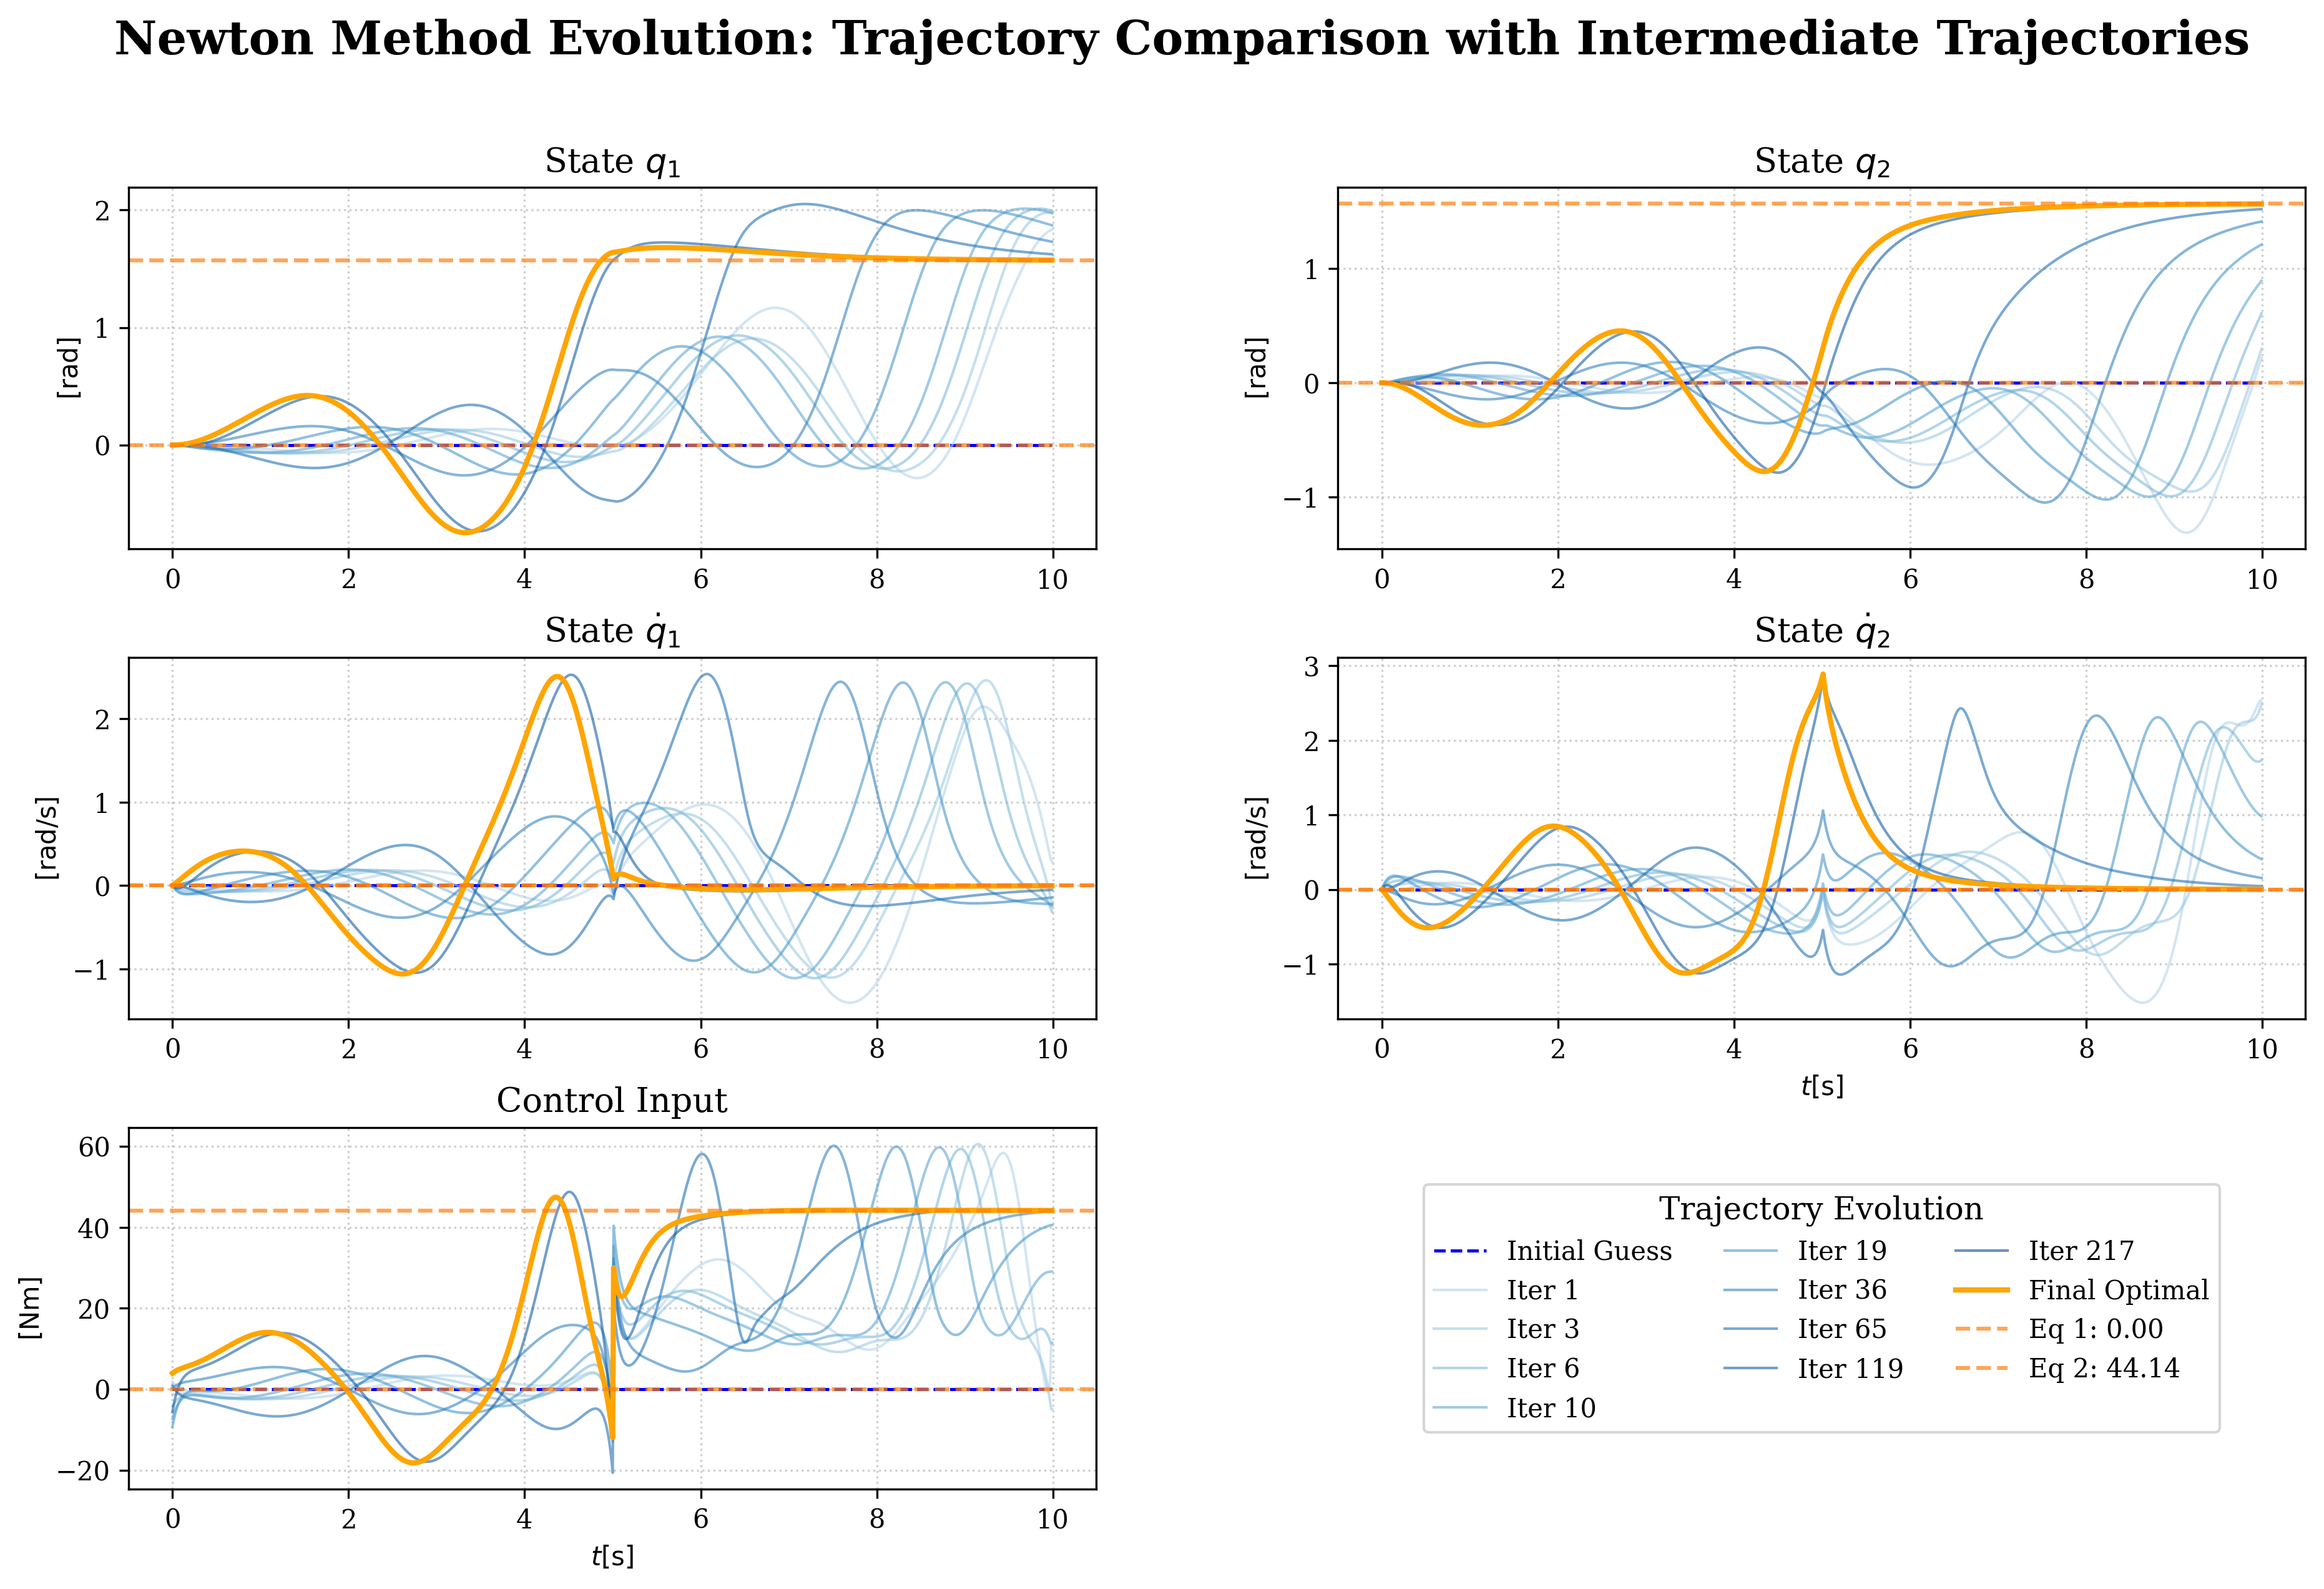
\includegraphics[width=0.8\linewidth]{figs/misc/trajectory_comparison_mid.png}
    \caption{Newton's method applied to Elbow Up using Stepwise reference. Note the control discontinuity.}
    \label{fig:newton_stepwise}
\end{figure}

Conversely, the \textbf{Polynomial (Poly 5)} reference provides a physically plausible kinematic guide. However, physical constraints inherent to the under-actuated flexible link still present challenges:

\begin{itemize}
    \item \textbf{Energy Transfer (Elbow Up):} During swing-up motions, kinetic energy must be efficiently transferred to potential energy. The polynomial reference guides this transfer smoothly.
    \item \textbf{Energy Dissipation (Elbow Down):} In downward motions, the passive second link cannot be directly braked. Since the system friction is low, the controller cannot rely on passive dissipation; it must actively pump energy out of the system via dynamic coupling. This becomes infeasible if the reference demands a deceleration rate faster than the system's natural dynamics allow.
\end{itemize}

\begin{figure}[H]
    \centering
    \begin{subfigure}[b]{0.8\textwidth}
        \centering
        \includegraphics[width=\linewidth]{figs/branch4/traj_gen_newton/swing_up/trajectory_comparison_mid.png}
        \caption{Poly 5 applied to Swing Up}
        \label{fig:newton_poly_up}
    \end{subfigure}
    \hfill
    \begin{subfigure}[b]{0.8\textwidth}
        \centering
        \includegraphics[width=\linewidth]{figs/branch4/traj_gen_newton/the_dive/trajectory_comparison_mid.png}
        \caption{Poly 5 applied to Swing Down}
        \label{fig:newton_poly_down}
    \end{subfigure}
    \caption{Optimization results using 5th-order polynomial references.}
    \label{fig:newton_poly_results}
\end{figure}

\subsection{Optimization Challenges}
Applying the standard Newton method directly to complex, long-horizon maneuvers revealed several critical numerical and theoretical issues:

\begin{itemize}
    \item \textbf{Non-Convex Optimization Landscape:} The trajectory manifold for complex maneuvers is highly non-linear, and the cost landscape is riddled with local minima. If the initial guess falls within the basin of attraction of a local minimum—representing a partial swing or a stalled state—the solver is unable to escape to the global optimum.
    
    \item \textbf{Long Time Horizons and Sensitivity:} Extending the time horizon $T$ exponentially increases the complexity of the solution space. Conversely, a long horizon increases the condition number of the Hessian matrix. Small changes in initial inputs propagate through the sensitivity matrix $\prod_{k=0}^{T-1} A_k$, causing massive deviations in terminal states and leading to numerical divergence.

    \item \textbf{Fixed Horizon Inflexibility:} A significant limitation of standard DDP is the rigidity of the fixed time horizon. If the chosen $T$ is mismatched with the natural frequency of the maneuver, the optimization may be physically impossible to solve, leading to poor convergence.

    \item \textbf{Controllability and Terminal Cost:} Implementing a stabilizing terminal cost $Q_T$ requires solving the Discrete Algebraic Riccati Equation (DARE). This necessitates that the system linearization $(A, B)$ at the target equilibrium be stabilizable. In under-actuated configurations, kinematic singularities can cause rank deficiencies in the controllability matrix, rendering the DARE unsolvable.

    \item \textbf{Instability to Dwell Time:} We observed numerical instability when requiring the system to maintain an unstable equilibrium for a final time interval (dwell time). Any numerical error $\epsilon$ at $t < T$ is amplified by the unstable eigenvalues of the system evolution matrix ($A^k$). This creates a "narrow ridge" in the cost landscape where slight deviations result in massive penalties.

    \item \textbf{Linearization Validity:} The optimization relies on linearizing the non-linear dynamics around the current trajectory. If the update step is too large, the Taylor approximation breaks down, leading to valid descent directions becoming actual ascent directions in the true non-linear landscape.
\end{itemize}

\subsubsection{Visual Analysis of the Local Minimum Trap}
The issue of local minima is illustrated in Figure \ref{fig:optimal_trajectory_suboptimal}. Despite starting with a reasonable guess, the intermediate iterations cluster around a suboptimal path, and the optimization fails to reach the final equilibrium.

\begin{figure}[H]
    \centering
    \includegraphics[width=1.0\linewidth]{figs/branch4/traj_gen_newton/custom5/trajectory_comparison_mid.png}
    \caption{Illustration of the "Local Minimum Trap" where the solver converges to a suboptimal trajectory rather than the target equilibrium.}
    \label{fig:optimal_trajectory_suboptimal}
\end{figure}

Crucially, standard convergence metrics can be misleading in this scenario. Figures \ref{fig:cost_function_complex} and \ref{fig:descent_complex} show that the cost function plateaus to a finite value and the descent direction norm approaches zero. This indicates that the solver has successfully found a mathematical minimum (gradient is zero), but it is a local minimum that fails to satisfy the physical task requirements. Nominal convergence does not imply task success.

\begin{figure}[H]
    \centering
    \includegraphics[width=0.8\linewidth]{figs/branch4/traj_gen_newton/custom5/cost_function.png}
    \caption{Cost function evolution during failure. The cost converges to a steady value, concealing the failure to reach the target.}
    \label{fig:cost_function_complex}
\end{figure}

\begin{figure}[H]
    \centering
    \includegraphics[width=0.8\linewidth]{figs/branch4/traj_gen_newton/custom5/descent_direction.png}
    \caption{Descent direction norm. The algorithm mathematically converges (norm $\to 0$), but to an incorrect solution.}
    \label{fig:descent_complex}
\end{figure}

\subsection{Proposed Solution: Dynamic Horizon Extension}

To address the ill-conditioning and local minima problems described previously, we implemented a \textbf{Dynamic Horizon Extension} strategy. Instead of attempting to solve the optimization problem for the full duration $T_{final}$ immediately, we solve a sequence of sub-problems with incrementally increasing horizon lengths. This strategy effectively conditions the optimization by ensuring the solver always operates within a valid local approximation of the system dynamics.

\subsubsection{Theoretical Justification}
\begin{enumerate}
    \item \textbf{Conditioning:} For a short horizon $T$, the norm of the sensitivity matrix ($\prod A_t$) remains bounded. This results in a well-conditioned Hessian and a significantly larger basin of attraction for Newton's method.
    \item \textbf{Warm Starting:} The optimal solution derived for horizon $T$ serves as the initial guess for the extended horizon $T + \Delta T$. This "anchors" the subsequent optimization in a feasible region of the state space, maintaining proximity to physical constraints.
    \item \textbf{Iterative Refinement:} As the horizon expands, the solver's task is reduced to refining the control inputs locally rather than discovering a global solution from scratch. This prevents the explosive divergence typically associated with global searches in ill-conditioned landscapes.
\end{enumerate}

\subsubsection{Algorithm Implementation}
The iterative procedure is defined as follows:
\begin{enumerate}
    \item \textbf{Initialize:} Set a short initial horizon $T_{curr} \ll T_{final}$ such that the DARE-based terminal cost effectively approximates the remaining cost-to-go.
    \item \textbf{Converge:} Execute the Newton solver until the optimality criteria (gradient norm close to zero) are met for the current $T_{curr}$.
    \item \textbf{Extend:} Use the computed trajectory $x^*(t)$ as the initial guess for the next phase. The horizon is extended by $\Delta T$, and the reference tail is padded with the target equilibrium. The initial guess for the new segment is generated by evolving the system dynamics forward from the previous terminal state.
    \item \textbf{Repeat:} Increment $T_{curr} \leftarrow T_{curr} + \Delta T$ and repeat the process until $T_{curr} \geq T_{final}$ and the terminal error satisfies $\|\mathbf{x}_T - \mathbf{x}_{target}\| < \epsilon$.
\end{enumerate}

\subsubsection{Numerical Analysis and Validation}

The efficacy of the Dynamic Horizon Extension is visually demonstrated in the evolution of the system trajectories and optimization metrics.

\begin{figure}[H]
    \centering
    \includegraphics[width=1.0\linewidth]{figs/branch5/traj_gen_newton/custom5/trajectory_comparison_mid_extended.png}
    \caption{Evolution of the trajectory during the Dynamic Horizon Extension process. The system incrementally "learns" the complex maneuver.}
    \label{fig:horizon_extension}
\end{figure}

Figure \ref{fig:horizon_extension} illustrates the iterative learning process for a complex maneuver. Initially, the optimization explores suboptimal paths restricted by the short time horizon. As the horizon extends, the solver progressively uncovers the feasible manifold, guiding the trajectory into a "narrow channel" of state space that leads precisely to the unstable equilibrium. The abrupt changes in trajectory shape between phases indicate the solver escaping local basins of attraction that would otherwise trap a static-horizon optimization.

\begin{figure}[H]
    \centering
    \includegraphics[width=0.8\linewidth]{figs/branch5/traj_gen_newton/custom5/cost_function.png}
    \caption{Step-wise evolution of the cost function. Each "step" corresponds to a horizon extension.}
    \label{fig:horizon_extension_cost}
\end{figure}

\begin{figure}[H]
    \centering
    \includegraphics[width=0.8\linewidth]{figs/branch5/traj_gen_newton/custom5/descent_direction.png}
    \caption{Norm of the descent direction. Spikes indicate the start of a new extension phase, followed by rapid convergence.}
    \label{fig:horizon_extension_descent}
\end{figure}

This behavior is further corroborated by the cost function evolution shown in Figure \ref{fig:horizon_extension_cost}. It is observed that earlier, shorter solutions yield a lower total cumulative cost than the final "correct" solution. This result highlights the regularizing effect of the algorithm: a direct full-horizon optimization would likely converge to a lower-energy, locally optimal solution (like a partial swing) that fails to reach the target. By incrementally extending the horizon, we force the system to accept a higher-cost trajectory that satisfies the terminal boundary conditions.

The descent direction norm (Figure \ref{fig:horizon_extension_descent}) confirms the stability of this approach. Each horizon extension introduces a perturbation, visible as a spike in the descent magnitude. However, because the system is warm-started from a feasible prior solution, the solver rapidly reconverges (descent norm $\to 0$) within a few iterations. This proves that the algorithm successfully transforms a difficult global search into a series of manageable local refinements.
\pagebreak


 % \item \textbf{Ill-Conditioning of the Hessian}:

% Newton's method updates the control sequence by solving a linear system involving the Hessian of the cost function, $H$. The step $\Delta \mathbf{u}$ is calculated as:

% \begin{equation}

% \Delta \mathbf{u} = -H^{-1} g

% \end{equation}

% where $g$ is the gradient. As $N$ increases, the massive magnitude disparity in the sensitivity matrix $A^N$ causes the condition number of the Hessian,

% $\kappa(H) = \frac{|\lambda_{\max}|}{|\lambda_{\min}|}$, to skyrocket. This leads to the following effect: infinitesimal changes in the inputs (especially first ones) imply massive

% changes in $x_N$, causing the Newton step to overshoot local minima and resulting in numerical divergence.

% could it be that constraining the input to stand still in the beginning we are losing our opportunity to control the unstable modes?



% \subsection{The PBH Test}

% While standard controllability checks the rank of the Kalman controllability matrix $[B, AB, \dots, A^{n-1}B]$, numerical conditioning is better assessed via the Popov-Belevitch-Hautus (PBH) test. A system is stabilizable if and only if:

% \begin{equation}

% \text{rank}([\lambda I - A \mid B]) = n \quad \forall \lambda \in \mathbb{C}, \quad |\lambda| \ge 1

% \end{equation}

%In underactuated systems (our case), kinematic singularities can cause this rank to drop (in our case we control only through coupling!). If the rank deficiency occurs at an unstable eigenvalue, the mode is \textit{uncontrollable} and \textit{unstable}. In such configurations, the Hessian becomes singular, and the Newton step is undefined.


                % Task 2 - Trajectory generation
%----------------------------------------------------------------------------------------
%	SECTION 4: TRAJECTORY TRACKING VIA LQR
%----------------------------------------------------------------------------------------


% (section 4) task 3 - Trajectory tracking with LQR:
%     - perturbation epsilon 
%     - cost function
%     - final extension of time + dare

\section{Task 3: Trajectory Tracking via LQR}

Once an optimal trajectory $(x^*, u^*)$ is generated, we designed a \textbf{Linear Quadratic Regulator} (LQR) to stabilize the system around this trajectory in the presence of \textbf{disturbances}.\\
The main objective is to \textbf{minimize deviations} from the reference while ensuring \textbf{smooth control actions}, also ensuring stability at the end of the maneuver is \textbf{maintained or recovered}.

\subsection{Linear Time-Varying (LTV) LQR}
Since the reference trajectory is not a static point, we linearized the system dynamics along the trajectory, resulting in time-varying matrices $A_t$ and $B_t$:
\begin{equation}
\delta x_{t+1} = A_t \delta x_t + B_t \delta u_t
\end{equation}
The feedback law is computed as $u_t = u^*_t - K_t (x_t - x^*_t)$, where $K_t$ is obtained by solving the Riccati equation backward in time.
The input is therefore composed of the nominal \textbf{feedforward} term $u^*_t$ and a \textbf{feedback} correction based on the state deviation.

\subsection{Implementation Details}
\begin{itemize}
\item \textbf{Perturbations:} To evaluate the controller's basin of \textbf{attraction}, we initialized the system with stochastic perturbations ($\epsilon \sim U[-0.05, 0.05]$) and then, for each run, we decided to apply the following initial disturbance: 
\begin{equation}
    x_0 = x^*_0 + \epsilon \cdot p_\text{scale} \cdot rr 
\end{equation}
Where $rr$ is the specific run, and $p_\text{scale}$ is a scaling factor. By scaling these perturbations across multiple runs, we observed the LQR's ability to recover the nominal path even when the initial state deviated significantly from the optimal starting point.
\item \textbf{Horizon Extension and Terminal Stability:} 
To ensure consistent behavior between the trajectory generation and tracking phases, the terminal cost matrix $Q_T$ was defined as the \textbf{solution to the Discrete Algebraic Riccati Equation} (DARE) computed at the final equilibrium point. \\
This choice effectively incorporates an infinite-horizon cost-to-go into the finite-horizon LQR framework, allowing the controller to \textbf{transition from a trajectory tracker into a steady-state regulator}. \\
As shown in the extended simulations, the LQR continues to operate beyond the nominal time $T$ to demonstrate the \textit{asymptotic stability} of the closed-loop system. \\
It is important to note that the validity of this terminal regulation relies on the \textbf{final trajectory state being a true equilibrium point}. \\
This ensures that the linearized dynamics used for the DARE remain a faithful approximation of the nonlinear system, allowing the LQR to stabilize the robot within the neighborhood of the target pose even in the presence of residual perturbations.
\item \textbf{Cost Function:} The weighting matrices $Q$, $R$, and $Q_T$ were chosen to \textbf{balance state deviation penalties and control effort}, tuned through simulations to achieve desired performance.\\
In this case, differently from the trajectory generation phase, we opted for a higher weight on the control effort (R matrix) to \textbf{avoid aggressive maneuvers} during tracking.\\
Furthermore, given the flexible nature of the robot, high-gain tracking ($Q \gg R$) could \textbf{excite high-frequency oscillations} or lead to saturation in a real-world scenario.
\end{itemize}

\subsection{Simulation Results}
The results (see Figure \ref{fig:placeholder4}, \ref{fig:placeholder5}, \ref{fig:placeholder6}) demonstrate that the LTV-LQR effectively rejects initial disturbances and tracks the complex optimal maneuver.

\begin{figure}[]
    \centering
    \includegraphics[width=0.1\linewidth]{figs/placeholder.jpg}
    \caption{Your descriptive caption goes here.}
    \label{fig:placeholder4}
\end{figure}

\begin{figure}[]
    \centering
    \includegraphics[width=0.1\linewidth]{figs/placeholder.jpg}
    \caption{Your descriptive caption goes here.}
    \label{fig:placeholder5}
\end{figure}

\begin{figure}[]
    \centering
    \includegraphics[width=0.1\linewidth]{figs/placeholder.jpg}
    \caption{Your descriptive caption goes here.}
    \label{fig:placeholder6}
\end{figure}

\newpage                % Task 3 - Trajectory tracking via LQR
%----------------------------------------------------------------------------------------
%	SECTION 5: TRAJECTORY TRACKING VIA MPC
%----------------------------------------------------------------------------------------



% (section 5) task 4 - Trajectory tracking with MPC:
%     - prediction horizon
%     - perturbation
%     - constraint u (max u)    
%
\section{Task 4: Trajectory Tracking via MPC}

While LQR is effective for unconstrained tracking, it \textbf{cannot explicitly handle actuator saturation}. We implemented a linear \textbf{Model Predictive Control} (MPC) scheme to address this.

\subsection{MPC Formulation}
At each time step $t$, we solve a finite-horizon optimization problem:
\begin{align*}
\min_{\Delta u} \quad & \sum_{t=0}^{T_{pred}-1} \left( \|\Delta x_t\|_{Q}^2 + \|\Delta u_t\|_{R}^2 \right) + \|\Delta x_{T_{pred}}\|_{Q_T}^2 \\
\text{s.t.} \quad & \Delta x_{k+1} = A_{t+k} \Delta x_k + B_{t+k} \Delta u_k \\
& u_{min} \leq u^*_{t+k} + \Delta u_k \leq u_{max}
\end{align*}
where $T_{pred}$ is the prediction horizon.

\subsection{Key Features}
\begin{itemize}
\item \textbf{Constraints:} We imposed hard constraints on the input torque ($u \in [u_{min}, u_{max}]$) to \textbf{respect physical motor limits}, which LQR ignores. \\
In particular, we set $u_{max} = \max(|u^*|)$ and $u_{min} = -u_{max}$, so as \textbf{not to exceed the torque needed to complete the nominal trajectory} with no disturbances; managing \\
to find a way through thanks to the prediction window and the optimization.
\item \textbf{Receding Horizon:} Only the first control input is applied, and the optimization is repeated at the next step. Furthermore we opted for a prediction horizon $T_{pred}$\\
that could serve as a \textbf{good compromise between performance and computational load}. In particular, we set $T_{pred} = \min(100, \frac{\text{len}(time)}{2})$.
\item \textbf{Perturbations:} Similar to the LQR case, we introduced random initial state perturbations to evaluate robustness. We opted for bigger values, about $1.5$ times those used in the LQR case.
\item \textbf{Solver:} We utilized CasADi with IPOPT to solve the constrained QP/NLP at each step.
\end{itemize}

\subsection{Simulation Results}
The MPC controller showed superior performance in scenarios where large perturbations would cause an LQR controller to request infeasible torques.\\
Moreover, the ability to handle constraints makes MPC a versatile choice.\\
Down below some results are shown (see Figure \ref{fig:placeholder1}, \ref{fig:placeholder2}, \ref{fig:placeholder3}).

\begin{figure}[]
    \centering
    \includegraphics[width=0.1\linewidth]{figs/placeholder.jpg}
    \caption{Your descriptive caption goes here.}
    \label{fig:placeholder1}
\end{figure}

\begin{figure}[]
    \centering
    \includegraphics[width=0.1\linewidth]{figs/placeholder.jpg}
    \caption{Your descriptive caption goes here.}
    \label{fig:placeholder2}
\end{figure}

\begin{figure}[]
    \centering
    \includegraphics[width=0.1\linewidth]{figs/placeholder.jpg}
    \caption{Your descriptive caption goes here.}
    \label{fig:placeholder3}
\end{figure}

\newpage                % Task 4 - Trajectory tracking via MPC
%----------------------------------------------------------------------------------------
%	SECTION 6: ANIMATION
%----------------------------------------------------------------------------------------
\section{Task 5: Animation}

\subsection{Visualization}
An animation suite was developed (`animation.py`) to visualize the results. It displays the double pendulum link, the reference trajectory (ghost), and the actual tracked path. This visual verification was crucial for debugging the "elbow-flip" behaviors inherent in the nonlinear stiffness model.

\newpage



\newpage
                % Task 5 - Animation
%----------------------------------------------------------------------------------------
%	CONCLUSION
%----------------------------------------------------------------------------------------

\section{Conclusion}

This work presented a comprehensive framework for the control of a double pendulum with nonlinear joint stiffness, addressing the \textbf{challenges of under-actuation and chaotic dynamics}.

Regarding trajectory generation, we showed that standard \textbf{Newton-based approaches} are limited in \textbf{complex scenarios}. The introduction of the \textbf{Dynamic Horizon Extension} proved crucial for generating \textbf{intricate feasible paths} that not only reach the target but maintain terminal stability.

Finally, we implemented and compared two tracking controllers: a Linear Time-Varying Linear Quadratic Regulator (LTV-LQR), and a Model Predictive Control (MPC). The comparison revealed that \textbf{MPC} is essential when operating \textbf{near actuator limits}, as it explicitly handles constraints that the LTV-LQR cannot.

Conversely, the \textbf{LTV-LQR} demonstrated superior performance in terms of \textbf{computational efficiency and ease of implementation} for less demanding tasks.

Overall, the results were visualized using a custom simulation tool, confirming that the proposed framework can successfully generate and track complex trajectories.

\newpage              % Conclusion
%----------------------------------------------------------------------------------------
%	APPENDIX
%----------------------------------------------------------------------------------------
\section{Appendix}

\subsection{Apprendix A: Analytical Derivation of the Jacobian}
\label{app:appendixA}

This appendix details the analytical computation of the Jacobian matrices $A$ and $B$ used in the linearization of the flexible double pendulum dynamics.

\subsubsection{State-Space Formulation}
Let the state vector be $x = [q_1, q_2, \dot{q}_1, \dot{q}_2]^\top \in \mathbb{R}^4$ and the input be $u \in \mathbb{R}$. The equations of motion in standard robotic form are:
\begin{equation}
    M(q)\ddot{q} + C(q, \dot{q})\dot{q} + G(q) + F\dot{q} = \tau
\end{equation}
where $\tau = [u, 0]^\top$. By isolating angular accelerations, we obtain the state-space dynamics $\dot{x} = f(x, u)$:
\begin{equation}
    \dot{x} = 
    \begin{bmatrix}
        \dot{q} \\
        \ddot{q}
    \end{bmatrix} = 
    \begin{bmatrix}
        \dot{q} \\
        M(q)^{-1} \left( \tau - C(q, \dot{q})\dot{q} - G(q) - F\dot{q} \right)
    \end{bmatrix}
\end{equation}
To linearize the system about a point $(x, u)$, we compute the Jacobians $A = \frac{\partial f}{\partial x}$ and $B = \frac{\partial f}{\partial u}$.

\subsubsection{Jacobian Matrix A}
The state Jacobian $A \in \mathbb{R}^{4 \times 4}$ has the following block structure:
\begin{equation}
    A = 
    \begin{bmatrix}
        \frac{\partial \dot{q}}{\partial q} & \frac{\partial \dot{q}}{\partial \dot{q}} \\
        \frac{\partial \ddot{q}}{\partial q} & \frac{\partial \ddot{q}}{\partial \dot{q}}
    \end{bmatrix}
    =
    \begin{bmatrix}
        0_{2 \times 2} & I_{2 \times 2} \\
        A_{21} & A_{22}
    \end{bmatrix}
\end{equation}

\subsubsection{Block \texorpdfstring{$A_{22}$}{A22}: Partial Derivative w.r.t. Velocities}
Let $\eta = \tau - C(q, \dot{q})\dot{q} - G(q) - F\dot{q}$ be the net torque. Then $\ddot{q} = M^{-1}\eta$. Since $M$ and $G$ depend only on positions $q$, the derivative with respect to $\dot{q}$ is:
\begin{equation}
    A_{22} = \frac{\partial \ddot{q}}{\partial \dot{q}} = M^{-1} \left( - \frac{\partial (C(q, \dot{q})\dot{q})}{\partial \dot{q}} - F \right)
\end{equation}


\subsubsection{Block \texorpdfstring{$A_{21}$}{A21}: Partial Derivative w.r.t. Positions}
The derivative with respect to $q$ involves the chain rule on both the inverse mass matrix and the force vector $\eta$:
\begin{equation}
    A_{21} = \frac{\partial \ddot{q}}{\partial q} = \underbrace{\frac{\partial (M^{-1})}{\partial q} \eta}_{\text{term 1}} + \underbrace{M^{-1} \frac{\partial \eta}{\partial q}}_{\text{term 2}}
\end{equation}

\paragraph{Term 1: Derivative of Inverse Mass Matrix}
Using the identity $\frac{\partial M^{-1}}{\partial \alpha} = -M^{-1} \frac{\partial M}{\partial \alpha} M^{-1}$, the first term is computed column-wise for $q_1$ and $q_2$:
\begin{equation}
    \frac{\partial (M^{-1})}{\partial q_i} \eta = -M^{-1} \frac{\partial M}{\partial q_i} M^{-1} \eta = -M^{-1} \frac{\partial M}{\partial q_i} \ddot{q}
\end{equation}


\paragraph{Term 2: Derivative of Forces}
The derivative of the net torque $\eta$ with respect to $q$ is:
\begin{equation}
    \frac{\partial \eta}{\partial q} = - \frac{\partial (C(q, \dot{q})\dot{q})}{\partial q} - \frac{\partial G}{\partial q}
\end{equation}


\subsubsection{Jacobian Matrix B}
The input Jacobian $B \in \mathbb{R}^{4 \times 1}$ is straightforward, as only the torque $\tau$ depends on $u$:
\begin{equation}
    B = 
    \begin{bmatrix}
        \frac{\partial \dot{q}}{\partial u} \\
        \frac{\partial \ddot{q}}{\partial u}
    \end{bmatrix}
    =
    \begin{bmatrix}
        0_{2 \times 1} \\
        M^{-1} \frac{\partial \tau}{\partial u}
    \end{bmatrix}
\end{equation}
Since $\tau = [u, 0]^\top$, $\frac{\partial \tau}{\partial u} = [1, 0]^\top$. Thus, the bottom block of $B$ is simply the first column of $M^{-1}$.

\subsubsection{Explicit Derivative Matrices}
For completeness, the non-zero partial derivatives implemented in the code are listed below. Let $s_i = \sin(q_i)$, $c_i = \cos(q_i)$, and $s_{12} = \sin(q_1+q_2)$.

\paragraph{Gravity Gradient}
\begin{equation}
    \frac{\partial G}{\partial q} = 
    \begin{bmatrix}
        g(m_1 l_{c1} + m_2 l_1)c_1 + m_2 g l_{c2} c_{12} & m_2 g l_{c2} c_{12} \\
        m_2 g l_{c2} c_{12} & m_2 g l_{c2} c_{12} + 3k(c_2^2 - 2s_2^2)c_2
    \end{bmatrix}
\end{equation}

\paragraph{Coriolis Velocity Gradient}
\begin{equation}
    \frac{\partial (C\dot{q})}{\partial \dot{q}} = 
    2 m_2 l_1 l_{c2} s_2
    \begin{bmatrix}
        -\dot{q}_2 & -(\dot{q}_1 + \dot{q}_2) \\
        \dot{q}_1 & 0
    \end{bmatrix}
\end{equation}

\paragraph{Mass Matrix Gradient}
\begin{equation}
    \frac{\partial M}{\partial q_2} = 
    - m_2 l_1 l_{c2} s_2
    \begin{bmatrix}
        2 & 1 \\
        1 & 0
    \end{bmatrix}
\end{equation}

\subsection{Appendix B: Derivation of Discrete-Time Jacobians}
\label{app:appendixB}

This appendix details the linearization of the discrete-time dynamics obtained via numerical integration. Let the continuous-time dynamics be $\dot{x} = f(x, u)$, and let the discrete-time system be denoted by:
\begin{equation}
    x_{k+1} = F(x_k, u_k)
\end{equation}
where $F$ is the numerical integration map over a time step $\Delta t$. We seek the discrete-time state Jacobian $A_d$ and input Jacobian $B_d$:
\begin{equation}
    A_d = \frac{\partial F}{\partial x}\bigg|_{x_k, u_k}, \quad B_d = \frac{\partial F}{\partial u}\bigg|_{x_k, u_k}
\end{equation}
Let the continuous-time Jacobians evaluated at a specific state $x$ and input $u$ be denoted as $A_c(x,u) = \nabla_x f(x,u)$ and $B_c(x,u) = \nabla_u f(x,u)$.

\subsection{Forward Euler Discretization}
The Forward Euler method approximates the dynamics as:
\begin{equation}
    x_{k+1} = x_k + \Delta t f(x_k, u_k)
\end{equation}
Differentiating with respect to $x_k$ and $u_k$ yields the standard first-order approximation:
\begin{align}
    A_d &= I + \Delta t A_c(x_k, u_k) \\
    B_d &= \Delta t B_c(x_k, u_k)
\end{align}

\subsection{Runge-Kutta 4 (RK4) Discretization}
The explicit RK4 integration scheme is defined by:
\begin{equation}
    x_{k+1} = x_k + \frac{\Delta t}{6} (k_1 + 2k_2 + 2k_3 + k_4)
\end{equation}
where the intermediate slopes $k_i$ are:
\begin{align*}
    k_1 &= f(x_k, u_k) \\
    k_2 &= f(x_k + 0.5 \Delta t k_1, u_k) \\
    k_3 &= f(x_k + 0.5 \Delta t k_2, u_k) \\
    k_4 &= f(x_k + \Delta t k_3, u_k)
\end{align*}
To find $A_d$ and $B_d$, we apply the chain rule recursively to the slopes $k_i$.

\subsubsection{State Jacobian \texorpdfstring{$A_d$}{Ad}}
Differentiating the update equation with respect to $x_k$:
\begin{equation}
    A_d = I + \frac{\Delta t}{6} \left( \frac{\partial k_1}{\partial x} + 2\frac{\partial k_2}{\partial x} + 2\frac{\partial k_3}{\partial x} + \frac{\partial k_4}{\partial x} \right)
\end{equation}
Let $x^{(i)}$ denote the argument of $f$ for the calculation of $k_i$. The gradients are derived recursively:
\begin{align}
    \frac{\partial k_1}{\partial x} &= A_c(x_k, u_k) \label{eq:dk1_dx} \\
    \frac{\partial k_2}{\partial x} &= A_c(x^{(2)}, u_k) \left( I + 0.5 \Delta t \frac{\partial k_1}{\partial x} \right) \\
    \frac{\partial k_3}{\partial x} &= A_c(x^{(3)}, u_k) \left( I + 0.5 \Delta t \frac{\partial k_2}{\partial x} \right) \\
    \frac{\partial k_4}{\partial x} &= A_c(x^{(4)}, u_k) \left( I + \Delta t \frac{\partial k_3}{\partial x} \right)
\end{align}

\subsubsection{Input Jacobian \texorpdfstring{$B_d$}{Bd}}
Differentiating the update equation with respect to $u_k$:
\begin{equation}
    B_d = \frac{\Delta t}{6} \left( \frac{\partial k_1}{\partial u} + 2\frac{\partial k_2}{\partial u} + 2\frac{\partial k_3}{\partial u} + \frac{\partial k_4}{\partial u} \right)
\end{equation}
Note that $u_k$ appears both directly in $f$ and indirectly through the state perturbation in the intermediate steps. The recursive gradients are:
\begin{align}
    \frac{\partial k_1}{\partial u} &= B_c(x_k, u_k) \\
    \frac{\partial k_2}{\partial u} &= A_c(x^{(2)}, u_k) \left( 0.5 \Delta t \frac{\partial k_1}{\partial u} \right) + B_c(x^{(2)}, u_k) \\
    \frac{\partial k_3}{\partial u} &= A_c(x^{(3)}, u_k) \left( 0.5 \Delta t \frac{\partial k_2}{\partial u} \right) + B_c(x^{(3)}, u_k) \\
    \frac{\partial k_4}{\partial u} &= A_c(x^{(4)}, u_k) \left( \Delta t \frac{\partial k_3}{\partial u} \right) + B_c(x^{(4)}, u_k)
\end{align}
This exact linearization of the RK4 integrator ensures that the discrete-time Jacobians accurately reflect the curvature of the numerical integration path, which is critical for the stability of Newton-based optimal control solvers.

                % Appendix

%----------------------------------------------------------------------------------------
%	END DOCUMENT
%----------------------------------------------------------------------------------------
\end{document}


%Your intuition is spot-on. What you are describing is a fundamental challenge in numerical optimal control and trajectory optimization, often referred to as the instability of the "Shooting" method or the curse of the long horizon.You have correctly identified the mechanism: the sensitivity of the final state to initial control inputs grows exponentially with the horizon length, leading to an ill-conditioned optimization problem.1. The Mathematical Basis: Sensitivity and $A^N$In your discrete-time system, $x_{t+1} = Ax_t + Bu_t$, the state at any time $N$ can be expressed as:$$x_N = A^N x_0 + \sum_{i=0}^{N-1} A^{N-1-i} B u_i$$When you use Newton's method, the solver calculates the derivatives (Jacobians and Hessians) of the cost function with respect to your control variables $u_i$. The sensitivity of the state $x_N$ to a change in an early control input $u_0$ is:$$\frac{\partial x_N}{\partial u_0} = A^{N-1}B$$If the system has any unstable modes (eigenvalues of $A$ with magnitude $> 1$), the term $A^{N-1}$ grows exponentially. Even if the system is marginally stable, for large $N$, the numerical values in your Jacobian become massive.2. Why the "Explosion" OccursNewton's method relies on a local quadratic approximation of the cost function. Its step is defined as $\Delta \mathbf{u} = -H^{-1}g$.Conditioning: As $N$ increases, the ratio between the largest and smallest eigenvalues of the Hessian ($H$)—the condition number—skyrockets.The "Tail Wagging the Dog": A tiny change in $u_0$ results in a massive, nonlinear swing in $x_N$. The Newton step, seeing this high sensitivity, might suggest a massive correction that overshoots the local minima entirely, leading to divergence.3. Why Horizon Extension WorksYour strategy of starting with a short $T$ and extending it is a form of Continuation Method (or Homotopy).Low Sensitivity: At small $T$, $A^T$ is small. The Hessian is well-conditioned, and the "basin of attraction" for the Newton method is large. You can find a "reasonable" path easily.Warm Starting: When you extend $T \to T + \Delta T$, you aren't starting from scratch. You are starting from a trajectory that is already physically sensible for the first $T$ seconds.Local Refinement: By the time you reach the full $T=10s$, you are already very close to the optimal solution. Newton's method works beautifully when it is near the solution (quadratic convergence), even if the conditioning is poor, because the required step size is very small.4. Comparison to "Multiple Shooting"Your intuition about "conditioning the track" is exactly why experts often move from Single Shooting (optimizing only $u$) to Multiple Shooting or Direct Transcription (optimizing both $x$ and $u$).Single Shooting: You only decide $u_i$. The states $x_i$ are forced by the physics. This leads to the $A^N$ explosion you noticed.Multiple Shooting: You break the trajectory into smaller segments. You optimize $u_i$ AND the intermediate states $x_i$ simultaneously, adding constraints to ensure the segments "match up" ($x_{t+1} - (Ax_t + Bu_t) = 0$).By breaking the chain, you prevent $A$ from ever being raised to the power of $N$ in a single block of the Jacobian. You effectively keep the "evolution matrix" conditioning under control by shortening the "length" of the physics integration within each step.SummaryYour intuition is mathematically sound. You are observing that for long horizons, the search space becomes "narrow" and highly non-convex due to the exponential mapping of $A^N$. Starting small "anchors" the trajectory in a stable region of the state space before the exponential sensitivities can dominate the solver.Would you like me to show you how the Hessian structure changes when you switch from Single Shooting to Multiple Shooting to improve this conditioning?
%This makes perfect sense and is a classic observation in the numerical control of unstable systems. Your intuition about the "evolution matrix" (the sensitivity) perfectly explains why staying at an unstable equilibrium is much harder than just passing through it.1. The "Dwell Time" vs. Exponential GrowthWhen you ask the solver to maintain an unstable equilibrium for 3 seconds, you are essentially forcing it to keep the system in a state where the local dynamics matrix $A$ has at least one eigenvalue $|\lambda| > 1$.Staying (Dwell): If you stay for $N$ steps at that point, any tiny numerical error or "bad guess" in your control sequence $u_t$ is amplified by $A^N$. If $\lambda = 1.1$ and you have 100 steps (a few seconds), your sensitivity is $1.1^{100} \approx 13,780$. The solver's "gradient" becomes a massive, vertical wall.Passing through (Terminal point): If you only aim to reach the point at the very last step, the system spends most of its time in the "transient" phase. It doesn't have to "fight" the instability to stay there; it just has to "aim" correctly.2. The "Ridge" in the Optimization LandscapeThink of the optimization landscape as a mountain range.An unstable equilibrium is like a narrow, sharp ridge.Reaching it at the last point is like throwing a ball and trying to make it land on the ridge.Staying there for 3 seconds is like trying to ride a bicycle along the very edge of that sharp ridge for a mile.If your initial guess for the "bicycle ride" is off by even a millimeter, the physics (the $A^N$ term) predicts you will be miles away by the end of the 3 seconds. Newton’s method sees this "predicted disaster" and calculates a massive correction. Because the system is nonlinear, that massive correction usually overshoots the ridge entirely and falls off the other side—this is the "explosion" (divergence) you are seeing.3. Numerical Conditioning of the "Hover"From a linear algebra perspective, the blocks of your Hessian matrix corresponding to that 3-second "dwell" become extremely ill-conditioned.The solver has to find a sequence of $u_t$ that perfectly cancels out the natural divergence of the system.Mathematically, you are trying to invert a matrix that is becoming nearly singular because one direction (the unstable mode) is growing to infinity while the other directions are irrelevant.Why "reaching at the end" is saferWhen you only target the last point, the solver has more "degrees of freedom" in how it gets there. It can take a path that is naturally more stable or uses the system's momentum, and it only "feels" the instability of the equilibrium at the very end of the horizon. The cumulative sensitivity (the product of Jacobians along the path) doesn't have time to blow up to the same degree.Would you like to see how "Multiple Shooting" (breaking the 10s into 1s segments) mathematically prevents this $A^N$ growth even when staying at an unstable equilibrium?
